\SubProblem
{مقایسه \lr{TDMA} و \lr{FDMA}}
{
پاسخ این سوال تقریبا مشابه پاسخ سوال قبلی است زیرا پایه روش‌ها یکسان است و فقط از آن‌ها برای حل دو مشکل متفاوت استفاده می‌کنیم.

\lr{TDMA}
روشی است که در آن کانال به اسلات‌های زمانی تقسیم می‌شود و هر اسلات به یک ارتباط داده می‌شود و اطلاعات آن ارتباط در آن اسلات‌های جابجا می‌شود.

\begin{itemize}
    \item
    این روش از پیش برنامه‌ریزی شده است پس هر ارتباط باید از آغاز شیار زمانی و موقعیت آن مطلع باشد.
    
    \item
    نیازمند همگام‌سازی است. برای اینکار از شیار محافظ اسفاده می‌کنیم.
    
    \item
     انتقال اطلاعات به صورت ناپیوسته و شکافته شده صورت می‌گیرد.
    
    \item
    برای سیگنال‌های صوتی مناسب است. برای فیلم و داده‌های با نرخ اطلاعات بالا مناسب نیست.
    
    \item
    هزینه ساخت و پیاده‌سازی کمتری دارد.

    \item
    نیازمند زمان‌بندی و هماهنگی دقیق است تا اسلات‌های زمانی با هم تداخل نداشته باشند و همچنین کانال بیکار نماند.
    
    \item
    استفاده از این روش در آنتن‌های خاص منظوره ساده‌تر است.
    
    \item
    هم به صورت متقارن و هم نامتقارن می‌توان آن را پیاده‌سازی نمود.
    
    \item
    در نسل‌های جدید تلفن همراه در کنار سایر روش‌ها بکار می‌رود.
    
    \item
    بهره‌وری در آن بیشتر از روش زیر است زیرا از کل ظرفیت کانال استفاده می‌کنیم.
    
    \item
    از نظر مصرف توان بهینه‌تر است.
    
    \item
    خیلی نیازمند پایداری و بهینگی سیگنال حامل نیست.
\end{itemize}

\begin{figure}[H]
    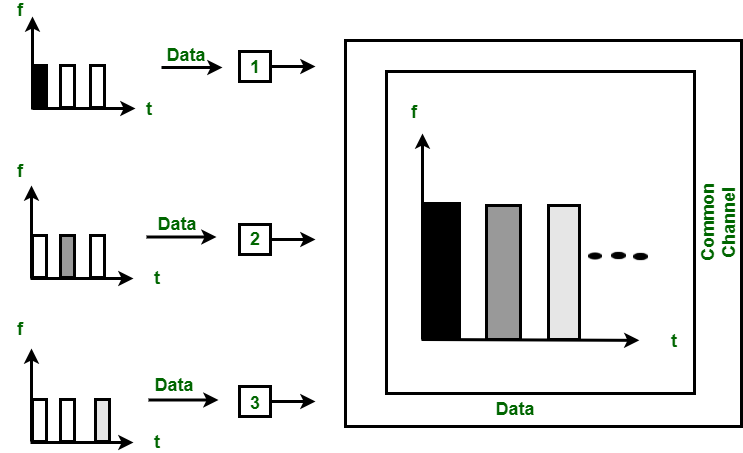
\includegraphics[width=12cm]{Images/TDMA.png}
    \centering
    \caption{\lr{TDMA}}
\end{figure}

\lr{FDMA}
روشی برای حل مشکل دسترسی چندگانه است که در آن پهنای باند به فرکانس‌های متفاوت تقسیم می‌شود و هر فرکانس در اختیار یک کاربر قرار می‌گیرد.

\begin{itemize}
    \item
    با مکانیزم تقسیم فرکانس کار می‌کند.
    
    \item
    نیازمند همگام‌سازی نیست.
    
    \item
    نیازمند باند محافظ
    \lr{(Guard Band)}
    است تا از تداخل جلوگیری کند.
    
    \item
    نیازمند
    \lr{Diplexer}
    پیچیده است و در کل روش پیچیده‌تری نسبت به روش زمانی است.

    \item
    استفاده از این روش در کنار روش
    \lr{MIMO}
    بسیار پیچیده است.
    
    \item
    استفاده از این روش در آنتن‌های خاص منظوره پیچیده است.
    
    \item
    از نظر مصرف توان کمتر بهینه است.
    
    \item
    نیازمند پایداری و بهینگی سیگنال حامل است.
    
    \item
    بیشتر در شبکه‌های
    \lr{GSM}
    و
    \lr{PDC}
    کاربرد دارد.
\end{itemize}

\begin{figure}[H]
    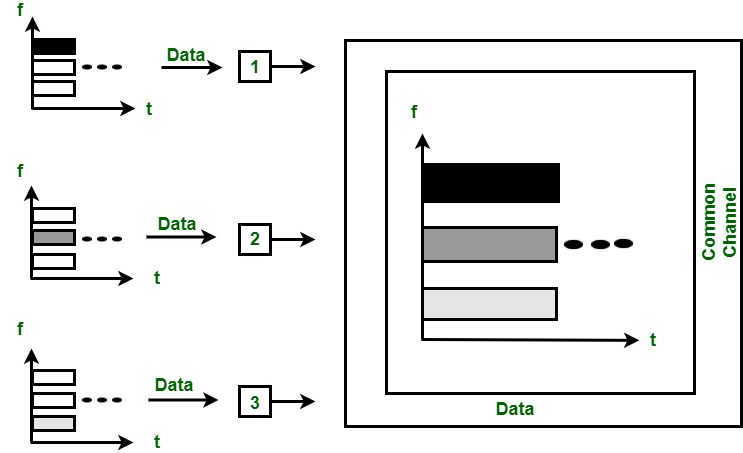
\includegraphics[width=12cm]{Images/FDMA.png}
    \centering
    \caption{\lr{FDMA}}
\end{figure}
}